\subsection{MILP Formulation}
\label{sec:MILP-selection-problem}
In this section we will derive algorithms for solving (\ref{eq:symbolic-optimization-with-minflow2}) that are taylored to a very specific case of the set $\mathcal{T}$.
% \subsubsection{Motivation: Coin Toss}
\begin{comment}
Consider again the stochastic process arising from a repetetive coin toss of example \ref{ex:tree-necessity}.
In order to translate this process into a numerical framework, we will assign the values 0 to heads and 1 to tails.
Here, the underlying space of events and values is discrete.
Generating a tree with values other than those encountered in the original stochastic process would not generate meaningful results.
This places a restriction on the space of allowable solution trees $\mathcal{T}$: 
The tree may only contain values that were part of the original set of scenarios.
\end{comment}
Consider a study on the robustness of a plane-based mail delivery system to cancellation of flights.
A large database of failures is available that can be used as data to form the initial stochastic process.
The next step is to generate a scenario tree from this data.
In order to evaluate the quality of a scenario tree, a metric for the space of all possible events is necessary.
This discrete space does not have a natural underlying metric space.
The metric must therefore be hand-crafted to fit this purpose.
For each pair of events, a \textbf{dissimilarity measure} must be provided.
Note that the tree generation algorithm will base its decision whether or not to aggregate scenarios o the values of the dissimilarity measure.
The modeling and optimization process therefore starts with this problem.

Another specialty of this problem is that generating a tree with values other than those encountered in the original stochastic process would not generate meaningful results.
This places a restriction on the space of allowable solution trees $\mathcal{T}$.
We denote this kind of problem as ``discrete-event''(DE) stochastic processes, as opposed to ``continuous-event''(CE) stochastic processes, for which intermediate values do make sense such as prices. CE processes will be discussed lateron in section \ref{sec:nlp}.

The restrictions added by the discrete nature of the value space turn problem (\ref{eq:symbolic-optimization-with-minflow2}) into a \textbf{selection problem}:
\begin{center}
  \textit{From the original set of scenarios, select nodes according to the tree structure, such that the Kantorovich Distance is minimized.}
\end{center}
It is generally possible to model the selection problem as an MILP. 
This full-size model, with far beyond 100,000 binary variables and a weak relaxation is, however, computationally intractable.
Several approaches will be explored that aim to overcome this complexity.

In a first attempt, the model will be decomposed by time steps, each of which is still modeled as an MILP.
The model will be solved using a state-of-the-art mixed integer programming solver.
Then it will be shown that the MILP can be solved with the K-medoids algorithm introduced in the previous section. This new approach will be shown to deliver extraordinary speedups.

In a third part, the shortcomings of the stage-wise approach are discussed.
Yet another algorithm is proposed, that aims to solve the full problem without stage decomposition using genetic optimization techniques.
This will be made possible by theorem \ref{thm:optimal-weights} on optimal weights.
Finally, some results for the methods are compared.
\begin{comment}
  \subsubsection{The Full MILP Model}
  Suppose we start with a (index) set $I$ of scenarios generated from the original stochastic process by sampling. For each node $k$ in the proposed tree structure, we introduce binary variables $z_{ki}$ which are 1 if node $k$ will take on the value of scenario $k$ of scenario $i \in I$ at the corresponding time step $t$, namely $\xi_i^t$. Using these variables, problem (\ref{eq:symbolic-optimization-with-minflow2}) can be formulated as the following MILP:
  \begin{eqnarray}
    % eta \in I \times I
    \label{eq:full-milp-objective}
    &\min\limits_{\eta, q, z}&\sum_{i\in I}\sum_{j\in J}\sum_{t\in T}\eta_{ijt}c(\xi_i^t,\xi_j^t)\\
    \label{eq:full-milp-qsum}
    &\mathrm{s.t.}&\sum_{i\in I}\eta_{ijt} = q_j\\
    \label{eq:full-milp-psum}
    &&\sum_{j\in J}\eta_{ijt} = p_i\\
    \label{eq:full-milp-q-distribution}
    &&q_j = \sum_{k\in \mathrm{children}(j)}q_k\\
    \label{eq:full-milp-tree}
    &&\eta_{ijt} \leq \eta_{i,\mathrm{father}(j),t-1}\\
    \label{eq:full-milp-only-selected}
    &&\eta_{ijt} \leq z_{kj} \\% Der fluss zu scenario j darf nur > 0 sein, wenn es fuer irgend eine node ausgewaehlt ist.
    \label{eq:full-milp-contibounds}
    &&0\leq q \leq 1,\;0\leq \eta \leq 1\\
    \label{eq:full-milp-binarybounds}
    &&z\in \left\{0,1\right\}
  \end{eqnarray}
  \todo[inline]{ist das modell wirklich korrekt so? }
  The probability measures $q_{jt}$ and $\eta_{ijt}$ are modeled as probabilities for each scenario $j\in J$ of the tree. 
  Each scenario corresponds to a leaf node.
  Equations (\ref{eq:full-milp-qsum}) and (\ref{eq:full-milp-psum}) represent the requirements on the marginal probabilities of the measure $\eta$ (see (\ref{eq:define-borel-measures})).
  Equation \ref{eq:full-milp-q-distribution} ensures the consistency of the probabilities of the nodes.
  The inequalities \ref{eq:full-milp-tree} are constraints that preserve the filtration of the original scenarios.
  With the inequalities \ref{eq:full-milp-only-selected}, all variables $\eta_{ijt}$ that belong to nodes $j$ that 

  The size of this mathematical program is prohibitively large. Common orders of magnitude for the cardinality of the set of scenarios is well above 1000. The tree size is dictated by the choice of $n_c$ and the time represented by the number of time steps $n_s$ one wants to look into the future. Even for very short times like $n_c=4$ and five branches to each node, the number of nodes quickly goes up to $n_N=155$. This leads to an MILP with $n_N\cdot n_s=155,000$, which means that it is computationally intractable. The intractability is not only due to the sheer size, but to the combination with the fact that the problem has a very weak relaxation.
\end{comment}
\subsubsection{Stage-Decomposition with MILP}
To reduce the complexity of the model, instead of solving all stages at the same time, we will solve the problem stage by stage. This greatly reduces the computational burden, because using the filtration constraints, we can solve the branches of the tree one at a time. These constraints allow us to 
\begin{enumerate}
\item solve the branch starting from each of the previously fixed nodes independently.
\item for the current branch starting at node $j$, discard all scenarios $i$ for which $\eta_{ij}=0$ in the problem corresponding to the father node of $j$.
\end{enumerate}

The algorithm for solving the stage-wise tree construction problem will be presented in the following.
\begin{algorithm}
  % \SetAlgoLined
  \KwIn{Set $I$ of $T$-stage scenarios $\xi_i^t$, tree structure $\mathcal{T}$}
  \KwOut{Scenario tree consisting of nodes $\nu_n$ and probobilities $q_j$}
  $F \leftarrow \{1\}$\tcc*{init set of father nodes with root node}
  $S_1 \leftarrow I$\tcc*{All scenarios share the root node}
  \While{$F\neq \emptyset$}{
    \ForEach{$f\in F$}{
      $F \leftarrow F\setminus \{f\}$\tcc*{remove this node from father set}
      Solve the MILP $\mathcal{M}_{sw}(f)$\;
      \ForEach{$k\in \{j\in S_f | z_j^f=1\}$}{
        Set value of next child of $f$ to $\xi_k^t$\;
        $S_k \leftarrow \{i\in S_f| \eta_{ik}^f>0\}$\;
        \If{$k$ has children}{
          $F \leftarrow F\cup \{k\}$\;
        }
      }
    }
  }
  $q_j\leftarrow $ optimal weights \tcc*{Using Algorithm \ref{alg:optimal-weights}}
  \caption{Stage-Wise MILP based Scenario generation}
  \label{alg:stage-wise-milp}
\end{algorithm}
%At every branching point, algorithm \ref{alg:optimal-weights} performs the search for the $n_c$ scenarios that best cover the distribution given by all scenarios that the current node in the previous stage was used to cover.

The procedure is outlined as algorithm \ref{alg:stage-wise-milp}.
The input is a set of scenarios $I$ defined over a set of stages $T$ and a tree structure $\mathcal{T}$, typically defined by the number of branchings of the tree at every node and timestep.
The distances $c(\xi_i^t, \xi_j^t)$ between the scenarios $\xi_i,\,\xi_j\; i,j\in I$ can be computed beforehand.
Note that the $1$-norm is the only meaningful norm that can be constructed this way, since the full distance is implicitly approximated as a sum over the stages.
For consistency, $c$ should therefore be chosen as the $1$-norm.
A set $F$ is used to keep track of the nodes for which can be solved next. Note that it is necessary to know the solution to the father node to be able to formulate the MILP $\mathcal{M}_{sw}(f)$ for a given node $f$. This set is initilized with the root of the tree. Additional sets $S_f\subset I$ are introduced for all $f\in F$. These sets hold all scenarios of the scenario set $I$ that are associated with the node $f$ through the transport variables $\eta$. Only the scenarios that had a non-zero ``mass-flow'' $\eta$ in the Kantorovich functional evaluation of their father node will be used in the construction of node $f$'s children in the tree. This property preserves the filtration information in the stage wise algorithm.

The problem that is solved for each father node $f$ in the previously defined tree is the following MILP:
\begin{eqnarray}
  \label{eq:small-milp-in-alg}
  \mathcal{M}_{sw}(f)\; \; \min_{\eta^f,z^f}&&\sum_{i\in I_f}\sum_{j\in I_f}\eta_{ij}^fc(\xi_i^t,\xi_j^t)\\
  \mathrm{s.t.}&&\sum_{j\in I_f}\eta_{ij} = \eta_{if}^{father(f)}\\
  &&\sum_{j\in I_f}z_j^f = n_c^f\\
  &&0\leq \eta_{ij}^f
\end{eqnarray}
The MILP models the decision which scenarios will be selected as nodes into the tree. Figure \ref{fig:swmilp-explanation} shows the evolution of the algorithm.
\begin{figure}
\centering
  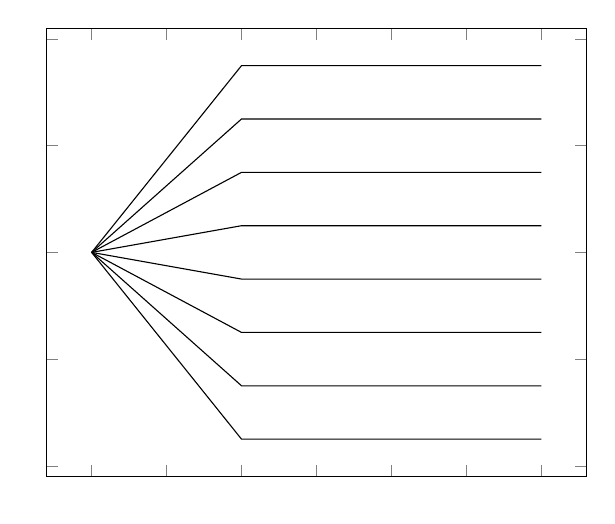
\begin{tikzpicture}
    \begin{axis}[xticklabels={,,},yticklabels={,,}]
      \addplot [color=black] coordinates {
        (1, 0)
        (2, -3.5)
        (3, -3.5)
        (4, -3.5)
      };
      \addplot [color=black] coordinates {
        (1, 0)
        (2, -2.5)
        (3, -2.5)
        (4, -2.5)
      };
      \addplot [color=black] coordinates {
        (1, 0)
        (2, -1.5)
        (3, -1.5)
        (4, -1.5)
      };
      \addplot [color=black] coordinates {
        (1, 0)
        (2, -0.5)
        (3, -0.5)
        (4, -0.5)
      };
      \addplot [color=black] coordinates {
        (1, 0)
        (2, 0.5)
        (3, 0.5)
        (4, 0.5)
      };
      \addplot [color=black] coordinates {
        (1, 0)
        (2, 1.5)
        (3, 1.5)
        (4, 1.5)
      };
      \addplot [color=black] coordinates {
        (1, 0)
        (2, 2.5)
        (3, 2.5)
        (4, 2.5)
      };
      \addplot [color=black] coordinates {
        (1, 0)
        (2, 3.5)
        (3, 3.5)
        (4, 3.5)
      };
    \end{axis}
  \end{tikzpicture}
  % begin of figure 2
  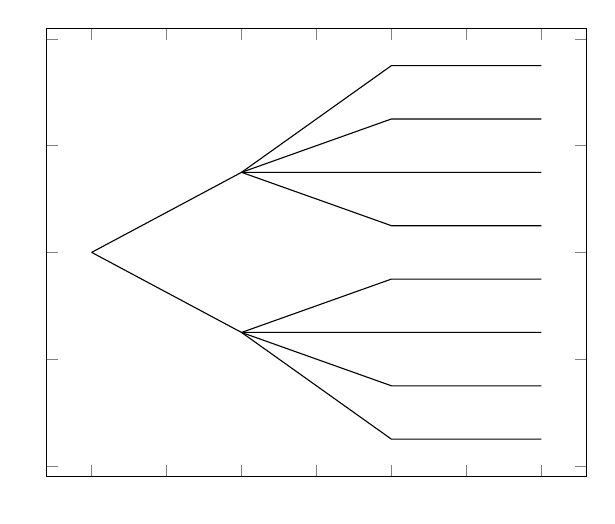
\begin{tikzpicture}
    \begin{axis}[xticklabels={,,},yticklabels={,,}]
      \addplot [color=black] coordinates {
        (2, -1.5)
        (3, -3.5)
        (4, -3.5)
      };
      \addplot [color=black] coordinates {
        (2, -1.5)
        (3, -2.5)
        (4, -2.5)
      };
      \addplot [color=black] coordinates {
        (1, 0)
        (2, -1.5)
        (3, -1.5)
        (4, -1.5)
      };
      \addplot [color=black] coordinates {
        (2, -1.5)
        (3, -0.5)
        (4, -0.5)
      };
      \addplot [color=black] coordinates {
        (2, 1.5)
        (3, 0.5)
        (4, 0.5)
      };
      \addplot [color=black] coordinates {
        (1, 0)
        (2, 1.5)
        (3, 1.5)
        (4, 1.5)
      };
      \addplot [color=black] coordinates {
        (2, 1.5)
        (3, 2.5)
        (4, 2.5)
      };
      \addplot [color=black] coordinates {
        (2, 1.5)
        (3, 3.5)
        (4, 3.5)
      };
    \end{axis}
  \end{tikzpicture}
  % begin of figure 3
  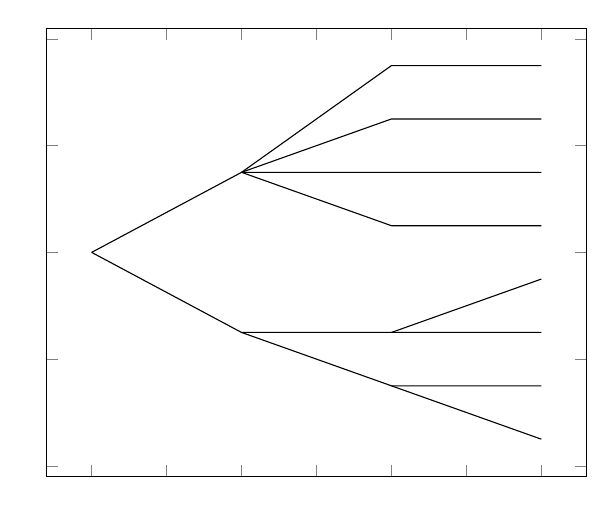
\begin{tikzpicture}
    \begin{axis}[xticklabels={,,},yticklabels={,,}]
      \addplot [color=black] coordinates {
        (3, -2.5)
        (4, -3.5)
      };
      \addplot [color=black] coordinates {
        (2, -1.5)
        (3, -2.5)
        (4, -2.5)
      };
      \addplot [color=black] coordinates {
        (1, 0)
        (2, -1.5)
        (3, -1.5)
        (4, -1.5)
      };
      \addplot [color=black] coordinates {
        (3, -1.5)
        (4, -0.5)
      };
      \addplot [color=black] coordinates {
        (2, 1.5)
        (3, 0.5)
        (4, 0.5)
      };
      \addplot [color=black] coordinates {
        (1, 0)
        (2, 1.5)
        (3, 1.5)
        (4, 1.5)
      };
      \addplot [color=black] coordinates {
        (2, 1.5)
        (3, 2.5)
        (4, 2.5)
      };
      \addplot [color=black] coordinates {
        (2, 1.5)
        (3, 3.5)
        (4, 3.5)
      };
    \end{axis}
  \end{tikzpicture}
  % begin of figure 4
  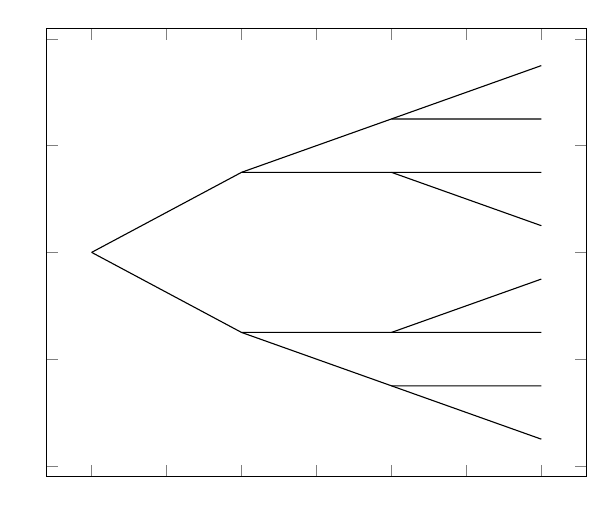
\begin{tikzpicture}
    \begin{axis}[xticklabels={,,},yticklabels={,,}]
      \addplot [color=black] coordinates {
        (3, -2.5)
        (4, -3.5)
      };
      \addplot [color=black] coordinates {
        (2, -1.5)
        (3, -2.5)
        (4, -2.5)
      };
      \addplot [color=black] coordinates {
        (1, 0)
        (2, -1.5)
        (3, -1.5)
        (4, -1.5)
      };
      \addplot [color=black] coordinates {
        (3, -1.5)
        (4, -0.5)
      };
      \addplot [color=black] coordinates {
        (3, 1.5)
        (4, 0.5)
      };
      \addplot [color=black] coordinates {
        (1, 0)
        (2, 1.5)
        (3, 1.5)
        (4, 1.5)
      };
      \addplot [color=black] coordinates {
        (2, 1.5)
        (3, 2.5)
        (4, 2.5)
      };
      \addplot [color=black] coordinates {
        (3, 2.5)
        (4, 3.5)
      };
    \end{axis}
  \end{tikzpicture}
  \caption{Evolution of the stage-wise MILP algorithm for a tree with two branches to each node.
    Top left: The tree is initialized with only the root node.
    Top right: After solving the MILP of the root node.
    Bottom left: After solving the lower of the two second stage nodes.
    Bottom right: The tree, completely solved.
  }
  \label{fig:swmilp-explanation}
\end{figure}
%%% Local Variables:
%%% mode: latex
%%% TeX-master: "da"
%%% End:
 % figure fig:swmilp-explanation
\subsubsection{Stage-Decomposition with K-medoids}
Even though the algorithm presented in the previous section is able to considerably reduce the computational burden of the problem, it still takes about 15 minutes to run on a dual core machine with 2500 Mhz and 4 Gbytes RAM, using Gurobi as the MILP solver.
Using theorem \ref{thm:kmeans-kantorovich}, a heuristic algorithm can be derived, that is an order of magnitude faster than the stage-wise MILP algorithm presented above.

Consider the above MILP $\mathcal{M}_{sw}(f)$ that is solved for every father node in the tree.
This MILP is the direct solution to problem \ref{prb:DE-Kantorovich-randvar} of finding the subset of events of a discrete random variable that form the best approximation.
With the help of theorem \ref{thm:kmeans-kantorovich} we can replace the solution of the MILP with the solution to the K-medoids problem.

There are many algorithms for solving the K-medoids problem.
For the purposes of this paper, a MATLAB implementation of the standard algorithm, ``Partitioning aroud Medoids''(PAM) was used \cite{Kaufman1987}.
PAM can be viewed as an implementation of algorithm \ref{alg:kmeans}, with a more specific maximization step. The details are not the concern here. The main point is that it can be computed orders of magnitude faster than the solution to the MILP and 

The adapted algorithm is presented as algorithm \ref{alg:stagewise-kmedoids}.
It follows along the same lines as the stage-wise MILP algorithm and uses the same sets $F$ and $S_k$.
The general evolution of the algorithm follows the one depicted in figure \ref{fig:swmilp-explanation}.
\begin{algorithm}
  \KwIn{Set $I$ of $T$-stage scenarios $\xi_i^t$, tree structure $\mathcal{T}$}
  \KwOut{Scenario tree consisting of nodes $\nu_n$ and probobilities $q_j$}
  $F \leftarrow \{1\}$\tcc*{init set of father nodes with root node}
  $S_1 \leftarrow I$\tcc*{All scenarios share the root node}
  \While{$F\neq \emptyset$}{
    \ForEach{$f\in F$}{
      $F \leftarrow F\setminus \{f\}$\tcc*{remove this node from father set}
      $[m,r] \leftarrow \operatorname{PAM}(K=n_c, X=\{\xi_i^t|i\in S_f\})$\;
      \For{$l=1\ldots n_c$}{
        $k \leftarrow child(f,l)$\tcc*{get child no. $l$ of node $f$.} 
        $\nu_k \leftarrow m_l$\;
        $S_k \leftarrow \{i | r_{ik}=1\}$\;
        \If{$k$ has children}{
          $F \leftarrow F\cup \{k\}$\;
        }
      }
    }
  }
  $q_j\leftarrow $ optimal weights \tcc*{Using Algorithm \ref{alg:optimal-weights}}
  \caption{Stage-wise $K$-Medoids}
  \label{alg:stagewise-kmedoids}
verfuegungverfuegung\end{algorithm}
\subsubsection{Stochastic Search Solution to Large-Scale MILP}
While the stage-wise methodology is an easy way to reduce the complexity of the problem, it may lead to an oversimplification. Figure \ref{fig:stagewise-failure} shows an example how stage-wise operating algorithms may yield arbitrarily bad tree approximations. 
\begin{figure}
  \centering
  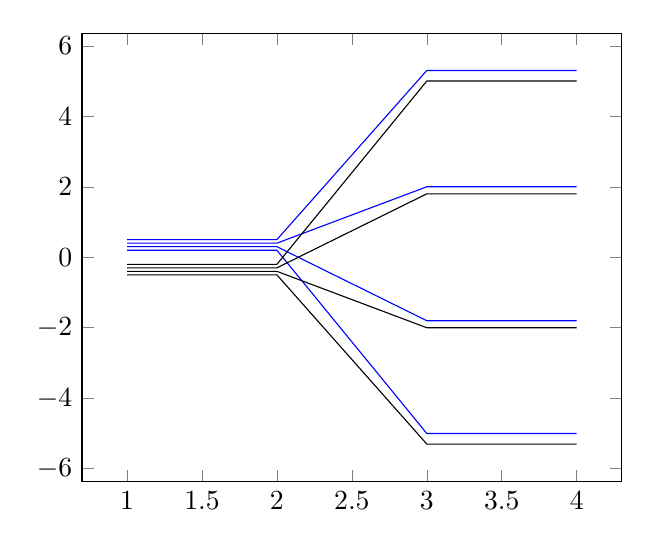
\begin{tikzpicture}
    \begin{axis}
      \addplot [color=blue] coordinates {
        (1, 0.2)
        (2, 0.2)
        (3, -5)
        (4, -5)
      };
      \addplot [color=blue] coordinates {
        (1, 0.3)
        (2, 0.3)
        (3, -1.8)
        (4, -1.8)
      };
      \addplot [color=blue] coordinates {
        (1, 0.4)
        (2, 0.4)
        (3, 2)
        (4, 2)
      };
      \addplot [color=blue] coordinates {
        (1, 0.5)
        (2, 0.5)
        (3, 5.3)
        (4, 5.3)
      };
      \addplot [color=black] coordinates {
        (1, -0.2)
        (2, -0.2)
        (3, 5)
        (4, 5)
      };
      \addplot [color=black] coordinates {
        (1, -0.3)
        (2, -0.3)
        (3, 1.8)
        (4, 1.8)
      };
      \addplot [color=black] coordinates {
        (1, -0.4)
        (2, -0.4)
        (3, -2)
        (4, -2)
      };
      \addplot [color=black] coordinates {
        (1, -0.5)
        (2, -0.5)
        (3, -5.3)
        (4, -5.3)
      };
    \end{axis}
  \end{tikzpicture}
  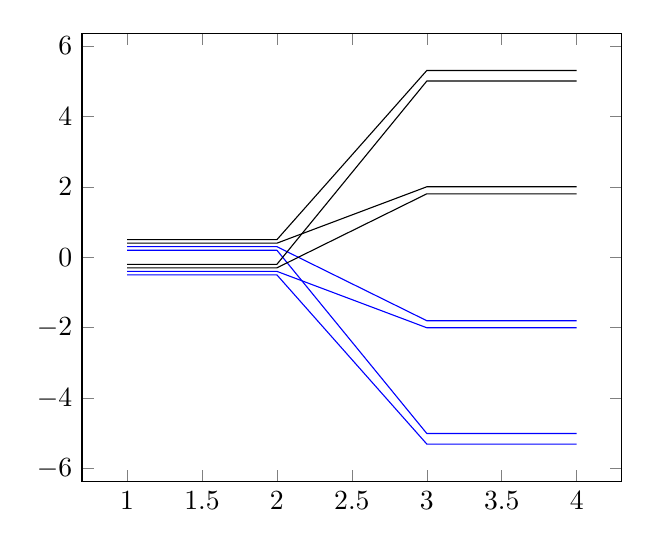
\begin{tikzpicture}
    \begin{axis}
      \addplot [color=blue] coordinates {
        (1, 0.2)
        (2, 0.2)
        (3, -5)
        (4, -5)
      };
      \addplot [color=blue] coordinates {
        (1, 0.3)
        (2, 0.3)
        (3, -1.8)
        (4, -1.8)
      };
      \addplot [color=black] coordinates {
        (1, 0.4)
        (2, 0.4)
        (3, 2)
        (4, 2)
      };
      \addplot [color=black] coordinates {
        (1, 0.5)
        (2, 0.5)
        (3, 5.3)
        (4, 5.3)
      };
      \addplot [color=black] coordinates {
        (1, -0.2)
        (2, -0.2)
        (3, 5)
        (4, 5)
      };
      \addplot [color=black] coordinates {
        (1, -0.3)
        (2, -0.3)
        (3, 1.8)
        (4, 1.8)
      };
      \addplot [color=blue] coordinates {
        (1, -0.4)
        (2, -0.4)
        (3, -2)
        (4, -2)
      };
      \addplot [color=blue] coordinates {
        (1, -0.5)
        (2, -0.5)
        (3, -5.3)
        (4, -5.3)
      };
    \end{axis}
  \end{tikzpicture}
  \caption{A stochastic process, for which algorithms that operate stagewise may yield arbitrarily bad results.
    The first plot shows the partition found by an algorithm which fixes the first stage before considering the second. 
    This yields a tree that is by far inferior to the one obtained by adjusting the tree to all stages at the same time}
  \label{fig:stagewise-failure}
\end{figure}
The MILP model for the full tree is, however, not computationally tractable.
In this section, we will present an algorithm based on genetic optimization techniques. 

When considering the full stochastic process at once, it is convenient to regard the scenarios as multidimensional events of a random variable. 
Recall from theorem \ref{thm:optimal-weights} that if the values of the nodes of the stochastic process are fixed, the Kantorovich distance o
\todo[inline]{Describe the stochastic search solution}
\todo[inline]{Create an algorithm object for the stochastic search solution}
\subsubsection{Results}
In this section, we will evaluate the scenario trees generated with the algorithms of the previous sections. As discussed above, the approach discussed in this part is particularly suitable to problems with a discrete set of outcomes at each stage. Therefore, we will focus on processes with that characteristic feature.
%
\paragraph{Implementations}
As all methods presented in this paper are new, the focus clearly lies on the derivation of the algorithms.
The results presented in this sections are based on ad-hoc implementations of these algorithms in MATLAB.
The MILP subproblems were solved using the commercial solver GUROBI.
The numbers on timing should be regarded only for a general orientation, and should not be judged on an absolute scale.
Many of the subalgorithms of the methods are of a heuristic or combinatorial nature.
Their performance is therefore susceptible to fine tuning, which was not conducted for the implementations.
Future implementations may therefore realize significant speedups through a better implementation of the same methods.
%
\paragraph{Testing methodology} 
Comparing scenario trees generated with different methods is not trivial.
The procedure we used to ensure relative reproducability of the results is as follows.
A set of scenarios was sampled from the original stochastic process.
This same set of scenarios was handed to each of the algorithms as input for the tree generation.
Using the same set of scenarios as input is important to not judge one of the tree generating algorithms for a singular event in its data scenarios.
The trees were then tested against ten new randomly generated sets of scenarios.
% The commercial solver Gurobi was employed to solve the MILP subproblems at each stage.
\paragraph{Coin Toss} Consider the stochastic process created by successive random coin tosses.
In order to analyze how well the algorithm does on unknown problems, we will pretend that the only information we have is a black box process that generates one scenario, which is a sequence of 3 successive coin tosses.
We, of course, know that the actual probabilities of each state.
We will compare the resulting scenario tree with
\paragraph{Log-normal SP}
\begin{figure}
  \begin{tikzpicture}
    \begin{axis} % time over number of scenarios 
      \addplot [color=black] coordinates {
        (500, 0.082675)
        (1000, 0.196757)
        (5000, 5.069326)
        (10000, 24.863489)
      };
    \end{axis}
    \end{tikzpicture}
    \begin{tikzpicture}
    \begin{axis} % 
      \addplot+[error bars/y dir=both, error bars/y explicit] coordinates {
        (500,  0.111438319659227) +- (0,0.003856365366939)
        (1000, 0.106969745621786) +- (0,0.001648309731920)
        (5000, 0.103710603975520) +- (0,0.000749656195408)
        (10000,0.103426137163199) +- (0,0.000595482018280)
      };
    \end{axis}
  \end{tikzpicture}
\caption{Results for Lognormal Distribution trees computed }
\end{figure}  
\begin{itemize}
\item the true solution, to assess the degree of suboptimality
\item with a naive tree generated by random selection of nodes from the set of scenarios. This helps us evaluate whether the extra effort put in to solve the MILP actually improved the prediction of the state.
\end{itemize}

%%% Local Variables: 
%%% mode: latex
%%% TeX-master: "da"
%%% End: 
